 %----------------------------------------------------------------------------------------
%	PACKAGES AND DOCUMENT CONFIGURATIONS
%----------------------------------------------------------------------------------------
\documentclass[11pt]{article}
\usepackage{subcaption}
\usepackage{amsmath} % Required for some math elements
\usepackage{hyperref} 
\usepackage[table,xcdraw]{xcolor}
\usepackage{lipsum} 
\usepackage{cite}
\usepackage{graphicx} % Required for the inclusion of images
\usepackage{algorithmic}
\usepackage{array}
\usepackage{bookmark}
\usepackage{listings}
\usepackage{amssymb}
\usepackage{enumitem}
\usepackage{pythonhighlight}
\usepackage[T1]{fontenc}
\usepackage{inconsolata}
\usepackage[margin=16mm]{geometry}
\usepackage{cleveref}

\newlist{steps}{enumerate}{1}
\setlist[steps, 1]{label = Step \arabic*:}

\hypersetup{ %color attributes of citation, link, etc.
    colorlinks=true,
    linkcolor=blue,
    filecolor=gray,      
    urlcolor=blue,
    citecolor=blue,
}

\newcommand{\matlab}{\textsc{Matlab }} %very important and totally necessary addition
\newcommand{\hdotrule}[1]{\hbox to \textwidth{\leaders\hbox to #1pt{\hss . \hss}\hfil}}

\newcommand\Item[1][]{%
  \ifx\relax#1\relax  \item \else \item[#1] \fi
  \abovedisplayskip=0pt\abovedisplayshortskip=0pt~\vspace*{-\baselineskip}}
%----------------------------------------------------------------------------------------
%	DOCUMENT INFORMATION
%----------------------------------------------------------------------------------------


\title{ECEN 405 -  D Class Amplifier \\ \large{\textit{``What a buck convertor would say if it could talk''}} }
\author{Daniel Eisen : 300447549 \\Team members: Niels Clayton \& Nickolai Wolfe}
\date{}

\begin{document}
\maketitle
\begin{center}
  \vspace*{-8mm}
  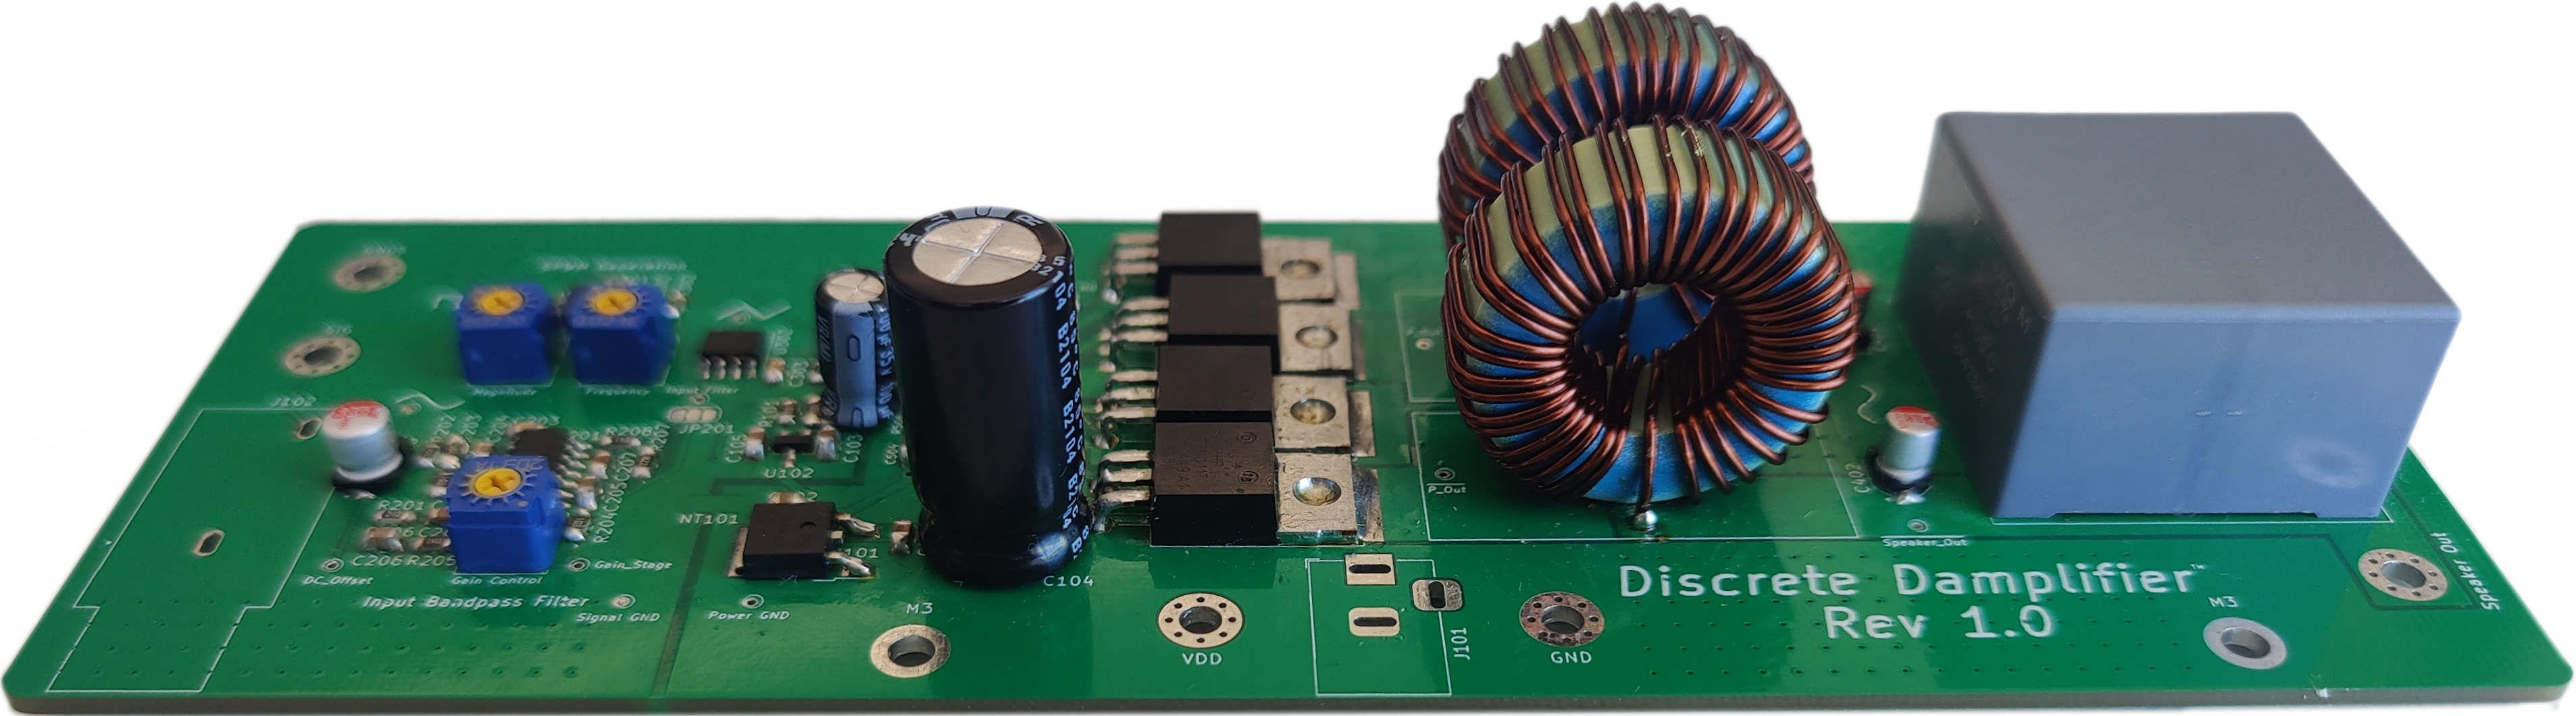
\includegraphics[width=0.75\textwidth]{img/real.png}
\end{center}{

\section{Introduction}

In the relm of auido amplifiers the D Class offers a method of supplying a high power loads with very high efficiency (esspecailly when compared to other classes). Classes A, AB offer high power output with very low signal distortion but suffer greatly in the efficency department due to continous linear conduction times and resulting losses in their amplifying elements/transistors. D class amplifiers can achieve up to 90-95\% power efficiency by taking advantage of a switching approach but require a more complex design process and circuit.

\begin{figure}[h!]
  \centering
  \frame{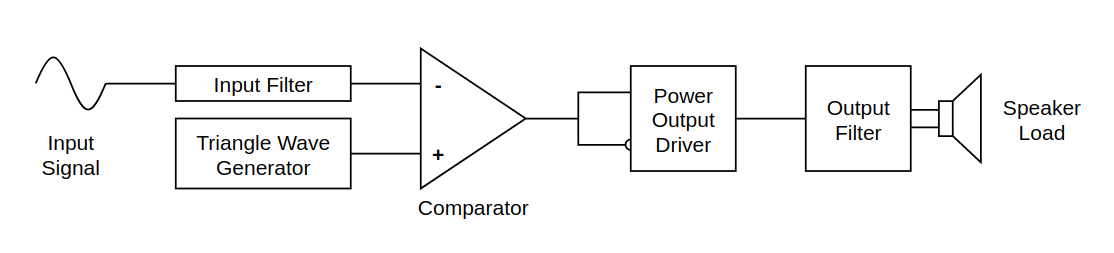
\includegraphics[width=0.8\textwidth]{img/D-class_block.png}}
  \caption{General Block Diagram of a D Class Amplifier}
  \label{F:block}
\end{figure}
A D class design can be broken up into and explain with a series of blocks illustrated above in \cref{F:block}. An input signal is sampled with a triangular wave into a high frequency SPWM carrier signal that is then amplified to high power by switching a MOSFET bridge and the carrier frequency is removed with a low pass filter. As the switching elements are either ON or OFF the continuous conduction losses near eliminated*.

This report outlines and discussed the specifics in design, implementation and results of constructing a D-class amplifier project to the specifications outlined below in \cref{S:spec}.

\subsection*{Specifications}\label{S:spec}
\begin{itemize}
  \item $P_{out}=80W$ for $R_{L} = 4\Omega$
  \item 10Hz to 200Hz Bandwidth
  \item Input sensitivity of 1V for maximum output (interpreted as 1V amplitude, 2V pk-pk)
  \item Maximum costs: \$50 per person
\end{itemize}

\section{Design}

A D-class amplifier operates on the signal sampling, switching amplification, and signal reconstruction as briefly described above. This project practically realised this approach with the high level design shown in \cref{F:top_schem}. 

\begin{figure}[h!]
  \centering
  \frame{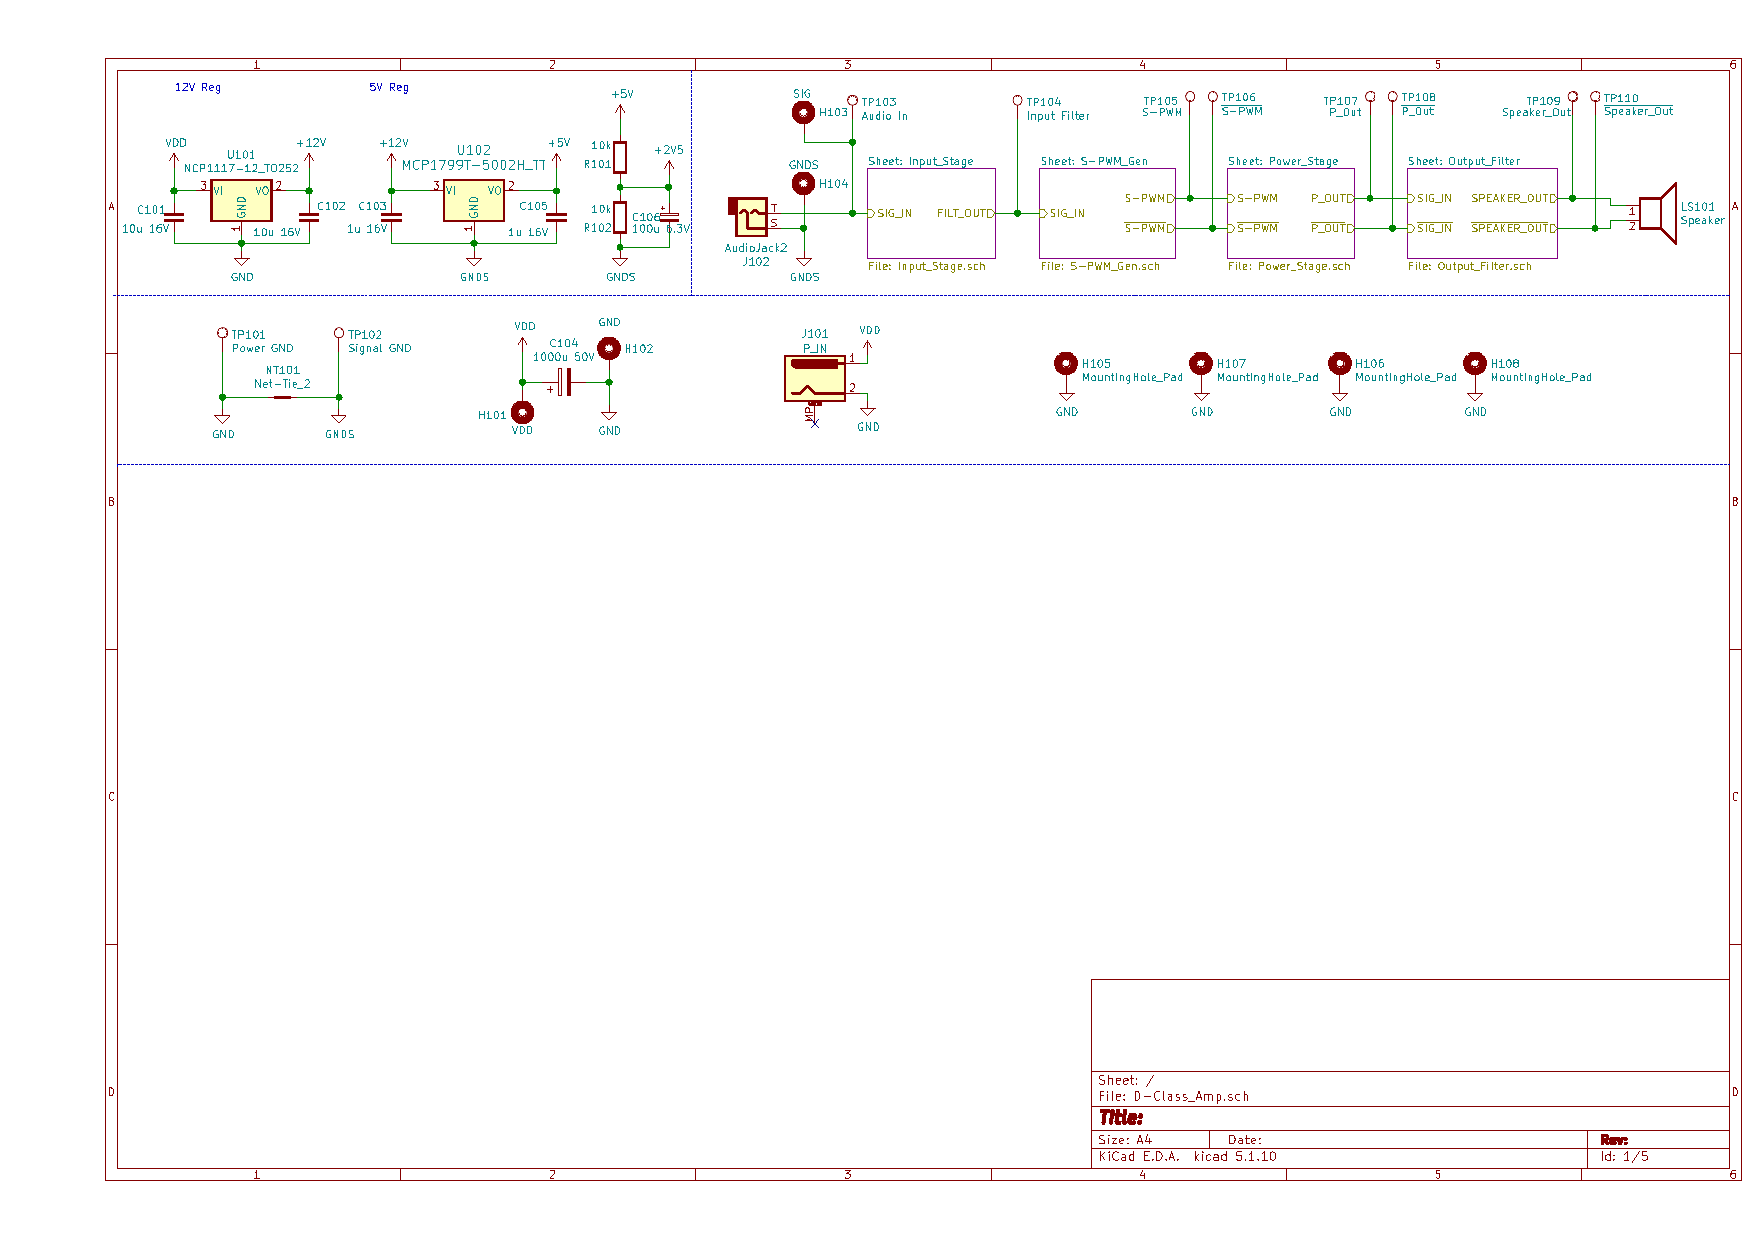
\includegraphics[page=1, trim={20mm 132mm 4.5mm 12.5mm},clip,width=0.85\textwidth]{img/schematic.pdf}}  \caption{Top Level Design Schematic}
  \label{F:top_schem}
\end{figure}

As the the intended load is a sub-woofer and there is a required bandwidth, the input audio signal must undergo some filtering and other preconditioning. This is handled by the input stage and was designed by Nickolai Wolfe. This stage band-passes the audio to meet the frequency range requirement, and otherwise adjusts gain and reference levels to make to suitable for the sampling stage.

The Sampler or Sinusoidal pulse width modulation (SPWM) generation stage was designed by Niels Clayton and encodes the audio signal into a high frequency carrier PWM signal. This signal is output (non-inverted and inverted for positive and negative output channel) at the correct voltage level for the driving circuitry as the switching control signal to the Power Amplifying Stage.

The last stage(s) of the D-Class is the Amplifying Bridges and reconstruction (Low pass) filters and their design was handled by myself. This project utilised two independent MOSFET bridges to amplify both SPWM signals and the reconstruction filter then strips out the high frequency carrier PWM to output the desired audio signal to the load.  

\subsection{Top Level Design Decisions}
\subsubsection*{Topology}
First is a topology choice. D-class amplifiers come in two main "flavours", Full and Half Bridge. Full Bridge amplifiers dedicate a whole bridge (1 driver, 2 MOSFETs) for each of a channels output rails. A Half bridge on the other hand has a single bridge that drives both the positive and negative sides of the output signal.

As the half bridge does not have independent bridges it will therefore require double the supply voltage (and is usually duel rail) to achieve the same output power. Its configuration also resulting in the commutation current being pumped back through the power supply, resulting in fluctuation and often the need for implementation a closed loop feedback system to maintain output stability. 

For the above drawbacks of the half-bridge as well as the fact that we are producing a mono output channel we decided to use an open loop full bridge topology to make breaking up the design simpler, maintain a single supply rail and sacrifice the required component duplication as a compromise. 

\subsubsection*{Power Supply}

Now that the project confirmed as Full Bridge, to meet the require output power to the 4 Ohm load the required VDD needs to be set.

\vspace*{-10mm}
\begin{align*}
  V_{DD} &= \sqrt{2\cdot R_{L}\cdot P_{out}} = 25.298V\\
         &= 26V (min)
\end{align*}

Another addition that was made as an extension to the scope the inclusion of 2 linear regulators to power the drivers and logic circuitry such that this project would produce a more cohesive final product. These are included in \cref{F:top_schem}.


\subsection{Input Bandpass Filter}

Nickolai designed the input stage that consists of 4th order Butterworth active low pass and a 2nd order active high pass filter with corner frequencies at 10Hz and 300Hz to meet the bandwidth specification in \cref{S:spec} with no attenuation at 200Hz. This stage additional imposes the signal on a mid-rail reference voltage of 2.5V to enable the entire logic side of this project to utilise a single ended 5V supply and also utilised a spare op-amp (from single quad package) as an adjustable gain stage for fine control and tuning.

All this is shown in \cref{F:ipf_schem} as the final design.

\begin{figure}[h!]
  \centering
  \frame{\includegraphics[page=2, trim={25mm 70mm 90mm 60mm},clip,width=0.85\textwidth]{img/schematic.pdf}}
  \caption{Input filtering schematic}
  \label{F:ipf_schem}
\end{figure}

\subsection{Audio Sampling and SPWM}

Niels designed the circuitry required to generate the high frequency triangle wave required to sample the processed input audio with the duel comparators to produced an inverted and non-inverted Sinusoidal Pulse-width-modulated signal at the required 5V level for controlling the gate drivers.    

\begin{figure}[h!]
  \centering
  \frame{\includegraphics[page=3, trim={35mm 133.5mm 30mm 15mm},clip,width=0.85\textwidth]{img/schematic.pdf}}
  \caption{Sampling triangle wave \& SPWM generation schematic}
  \label{F:sample_schem}
\end{figure}

It basically operates by comparing the current signal level to the triangle wave and encoding that in the width of the SPWM. This circuit also integrates both adjustable triangle wave frequency and scale to tune the switching speed and signal enveloping for best performance.

\newpage
\subsection{Power Stage and Output Filter}

These sections are required to amplify the generated 5V SPWM from the sampler filter out the carrier frequency to reproduce the audio signal. 

They consist of two symmetric MOSFET bridges (non-inverted and inverted SPWM amplifiers) that forming the full bridge topology and a low pass reconstruction filter to decode the audio signal.
Each of these require require following a design procedure to meets specification and the optimisation of component choice to minimise losses, maintain signal integrity and add protection.

\subsubsection*{Power Amplifying Bridge}\label{S:power_des}

In order the successfully amplify the SPWM encoded audio the MOSFET bridges must be switched quickly and efficiently, minimising conduction losses and retaining signal clarity. The design of such an effective amplifying bridge relies on three main aspects: 

\begin{itemize}
  \item Correct MOSFET Selection
  \item Gate Drivers for fast gate charging
  \item Bootstrapping and switching dead time
\end{itemize}

The finalised design of both bridges is shown here in \cref{F:gate_drive_schem} accepting the 5V SPWM signals and outputting the POUT amplified signal for filtering.

\begin{figure}[h!]
\centering
\frame{\includegraphics[page=5, trim={85mm 149mm 5mm 12mm},clip,width=0.85\textwidth]{img/schematic.pdf}}
\caption{Gate driver schematic}
\label{F:gate_drive_schem}
\end{figure}

Before component selection can occur the FET voltage rating must be calculated:

\begin{align}
  BV_dss &= \frac{\sqrt{2\cdot P_{out}\cdot R_{L}}}{0.85}\cdot1.5 = 44.6V
\end{align}

The selected FETs for the project are the PHP23NQ11T. These were selected for their combination of very low $R_ds(on)$ of $49m\Omega$ and very low gate charge of $10nC$. These factors work to minimise gate charge time as well as reduce the on state conduction power loss. They exceed the voltage rating at 110V and have an ambient power dissipation of 100W so will be comfortably operating at maximum quarter power. 

The IR21834PBF in SMD packaging were selected as the gate driving ICs as they integrate a large all the necessary features for proper bridge control. Each is a dedicated half-bridge driver designed of the required bootstrap operation to properly reference the high-side MOSFET to allow for successful switching. It can supply the gate outputs with up to 1.8A of charge current for nominal gate ON/OFF times of 40ns and 20ns. It is also 5V input to be compatible with the SPWM generation stage and features a matched preparation delay between each channel to prevent phase drift/offset and inter-channel interference in the filter stage.  

Most importantly these drivers support a programmable dead time to prevent VDD to GND shoot through across the FETs and allows for tuning the project overall THD by changing the control resistance, nominally set to 10K for a 63nS dt.

\subsubsection*{Reconstruction Filter}

This D-class is designed around a minimum switching/carrier frequency of 30kHz therefore a filter is required on the bridges output to attenuate this and restore the audio signal for output and driving the sub-woofer. Even though the carrier frequency is outside the audible range and the sub-woofer could not accurately reproduce it, leaving it unfiltered could degrade the efficiency and well as cause EMI issues.

As audio signal integrity is a priory the chosen topology is a low-pass Butterworth filter to maintain a flat gain in the passband and good phase response.
Specifically the configuration chosen is the Alternate Balanced 2-Pole Filter shown in \cref{F:opf_schem}. This utilises duel matched inductors ($L$) to eliminate common-mode swing, a single full rail unpolarised capacitor ($C_L$) for improved rejection and two addition balancing capacitors ($C_{a,b}$) that provide a HF ground shorts.

\begin{figure}[h!]
  \centering
  \frame{\includegraphics[page=4, trim={115mm 97mm 105mm 75mm},clip,width=0.5\textwidth]{img/schematic.pdf}}
  \caption{Alternate Balanced 2-Pole LPF}
  \label{F:opf_schem}
\end{figure}

The calculation of these values are all derived from the load ($R_L$) and selected cutoff frequency. This was placed one decade before the minimum switching frequency of 30kHz to ensure a -40dB attenuation.

\begin{align}
    f_{0} &= 3\,kHz, \; \omega_{0} = 18850\,rad.s^{-1} \\
    C_{L} &= \frac{1}{R_{L}w_{o}\sqrt{2}} = 9.38\,\mu F \\
  C_{a,b} &= 0.2C_{L} = 1.88\,\mu F \\
        L &= \frac{R_{L}\sqrt{2}}{2w_{o}} = 150\,\mu H
\end{align}

These exact values are obviously not directly available for purchase and obtaining the inductors is the main limiting factor. Therefore the above values were used as the starting off point in component selection, and the recalculated values to match the available inductors were simulated to ensure functionality was retained. 

\begin{figure}[h!]
  \centering
  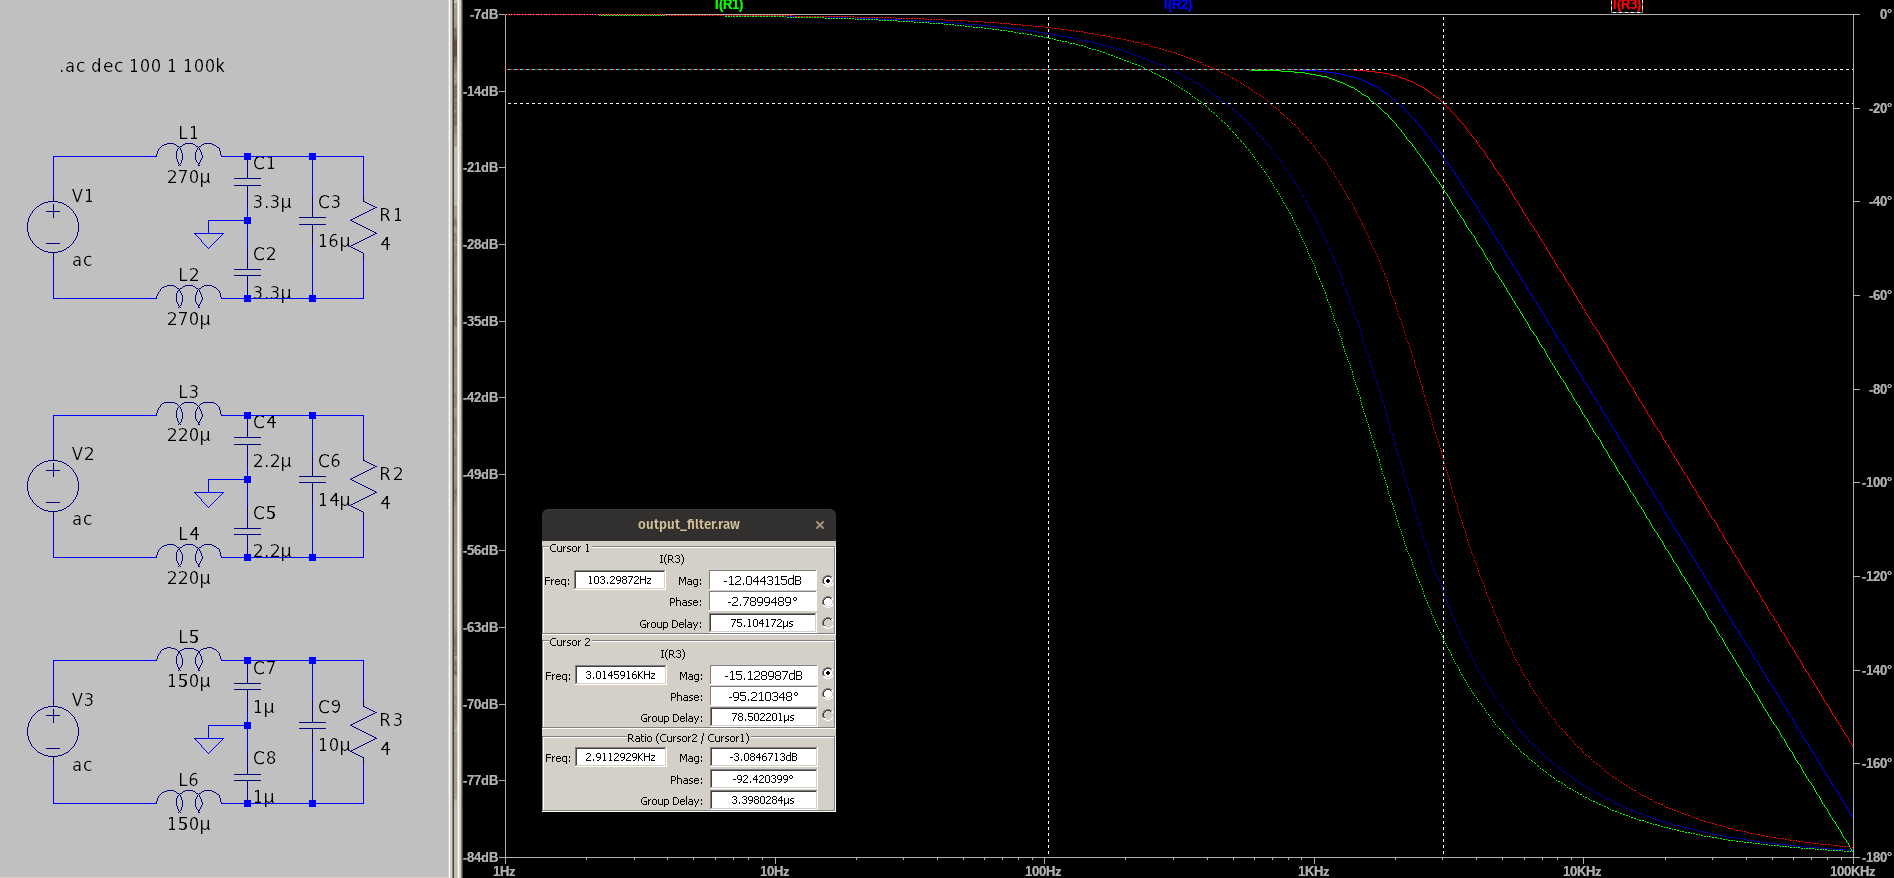
\includegraphics[width=0.6\textwidth]{img/output_filter_sim.png}
  \caption{Output filter option simulations}
  \label{F:opf_sim}
\end{figure}

In \cref{F:opf_sim} you can see the 3 real world attainable circuits (based of real component values in stock) simulated. These all still match in topology performance and all have a corner frequency (-3dB) of under 3kHz thus retaining the intended attenuation.
All these values were found in the same or very similar product series. The inductors were sourced as high current (5A), shielded core signal transformers to ensure a constant inductance across the expected output current, the main capacitor was a unpolarised film capacitor for signal quality, tight tolerances and closer to ideal characteristics.

From these the final values were selected to help meet the price specification.

\section{Implementation}
\subsection{PCB Layout}

With each of the amplifiers stages fully designed and top-level connective schematic complete, the next step is to implement it by laying out an integrated PCB. This can be seen in \cref{F:PCB} showing the full layout the projects deliverable.

\begin{figure}[h!]
  \centering
  \begin{subfigure}{0.45\textwidth}
    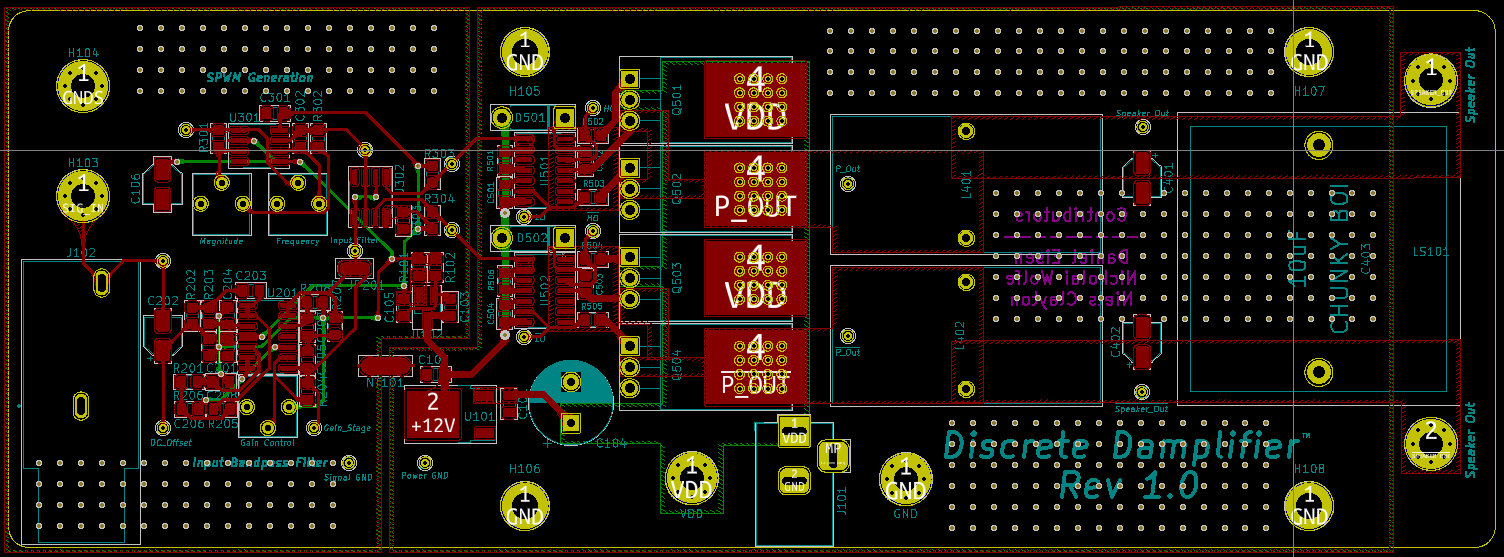
\includegraphics[width=\columnwidth]{img/traces.png}
    \subcaption{PCB trace layout}
  \end{subfigure}
  \begin{subfigure}{0.45\textwidth}
    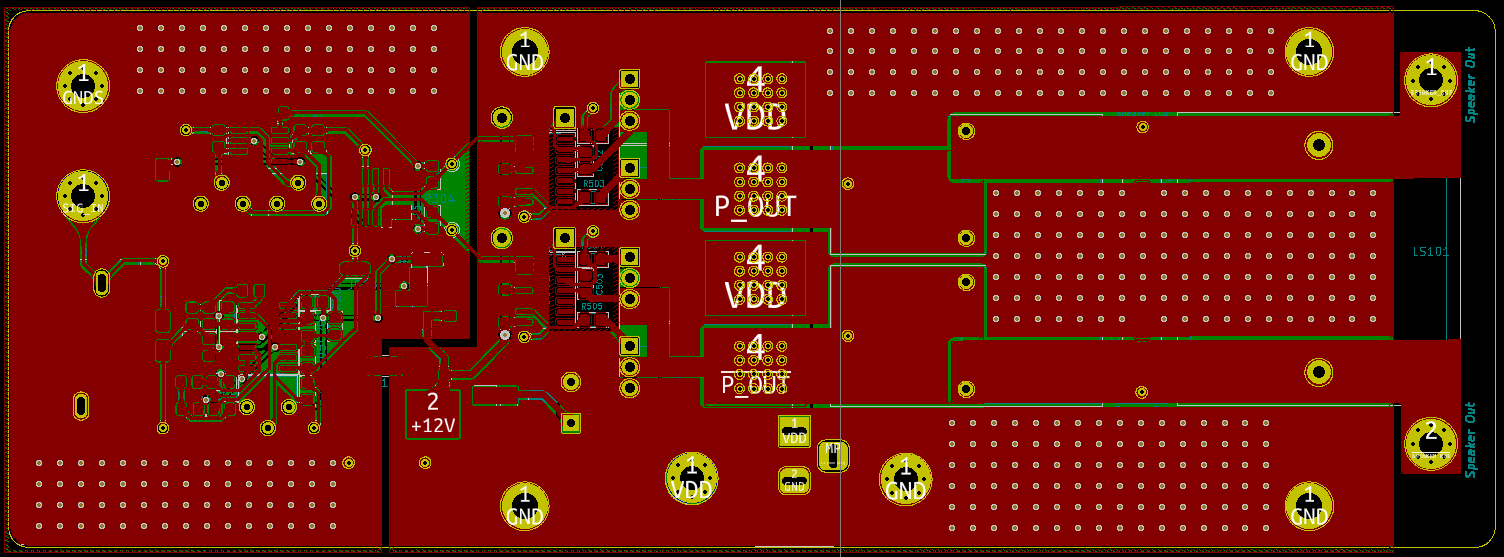
\includegraphics[width=\columnwidth]{img/top_layer.png}
    \subcaption{Top Copper}
  \end{subfigure}
  \begin{subfigure}{0.45\textwidth}
    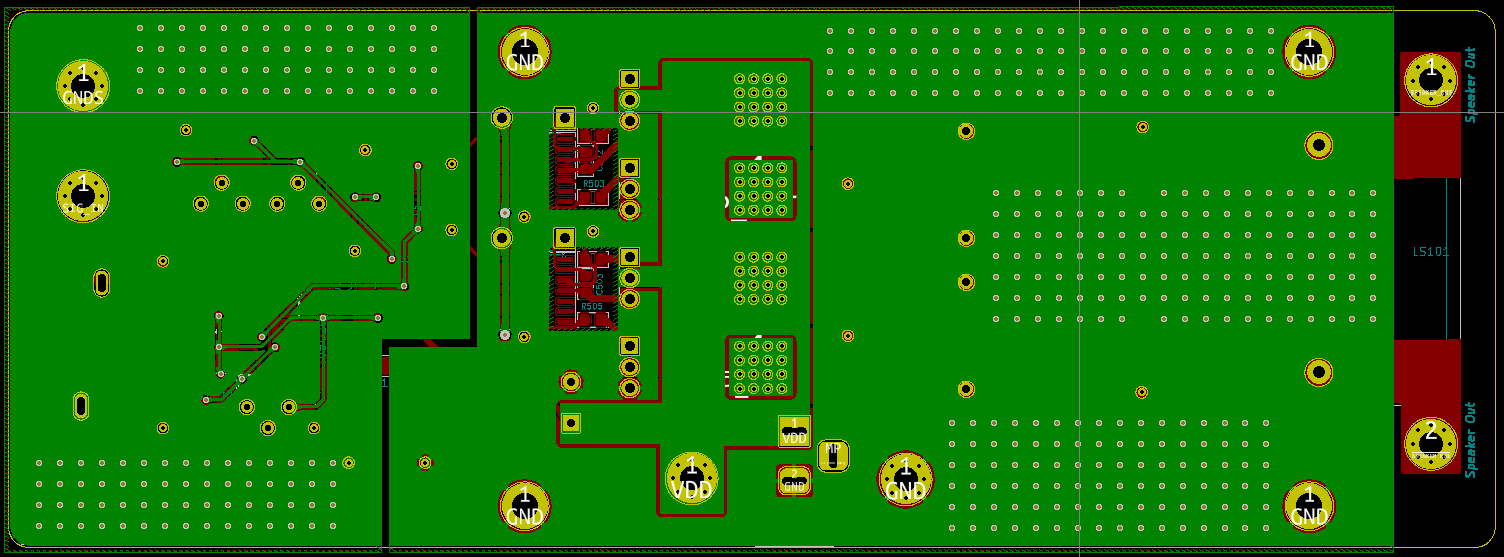
\includegraphics[width=\columnwidth]{img/bottom_layer.png}
    \subcaption{Back Copper}
  \end{subfigure}
  \caption{Final Full PCB}
  \label{F:PCB}
\end{figure}

By design this project includes a mix of sensitive signal processing at the input, and high power, high frequency switching at the output. This represents and important requirement to isolation of grounds and management of current return paths.

This is primarily achieved by completely separating the Power and Signal ground planes on both sides and providing a single return path for signal currents to  via a net-tie from signal to power ground. This completely prevents any high currents from the amplification bridges from returning around/under the sensitive op amps. \Cref*{F:PCB} b\&c's copper pour shows this isolation and return path.

Adjacent to this approach, this project heavily utilised copper pour zones and heavy via stitching to ensure constant ground references and very low impedance current paths for the high power output. To match these custom zones we also made custom FET footprints that allows us to dissipate excess heat into the board.

Finally we defined explicit pour keepout zones under the output terminals to prevent connectors shorting to the ground plane and under the output half both gate drivers to prevent noise coupling into the gate input signals.

\subsection{Gate Driving and Bridge Output}
\begin{figure}[h!]
  \centering
  \begin{subfigure}{0.3\textwidth}
    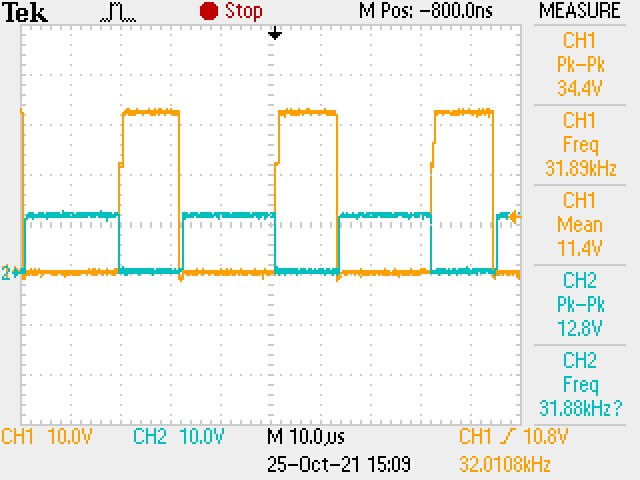
\includegraphics[width=\columnwidth]{img/testing/power_output/gate_input.JPG}
    \subcaption{High and Low side gate signals}
  \end{subfigure}
  \begin{subfigure}{0.3\textwidth}
    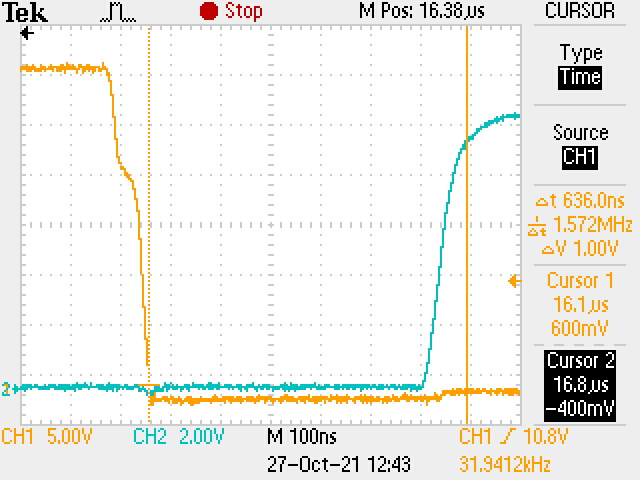
\includegraphics[width=\columnwidth]{img/testing/power_output/dead_time.JPG}
    \subcaption{Deadtime}
  \end{subfigure}
  \begin{subfigure}{0.3\textwidth}
    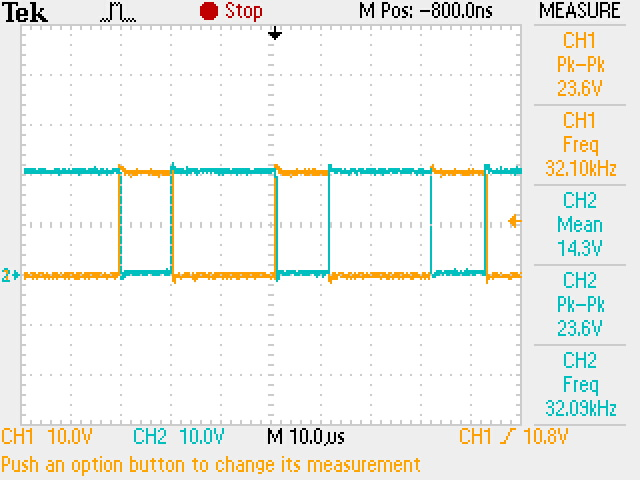
\includegraphics[width=\columnwidth]{img/testing/power_output/fet_output.JPG}
    \subcaption{Both bridges amplified SPWM (FET outputs)}
  \end{subfigure}
  \caption{}
  \label{F:imp_drive}
\end{figure}

The bridge driving sections functionality was confirmed by examining the generated gate signals, dead-time and the resulting amplified signals. In \cref{F:imp:drive} you can observe the high side gate signal (a) being correctly bootstrapped up and the Miller charge plateau can even be seen, the deadtime (b) is also successfully being set at 63ns as outlined in  \cref{S:power_des}, and successfully results in a non-inverted and inverted amplified SPWM (c).

\subsection{Reconstruction Filter}
 
\begin{figure}[h!]
  \centering
  \begin{subfigure}{0.3\textwidth}
      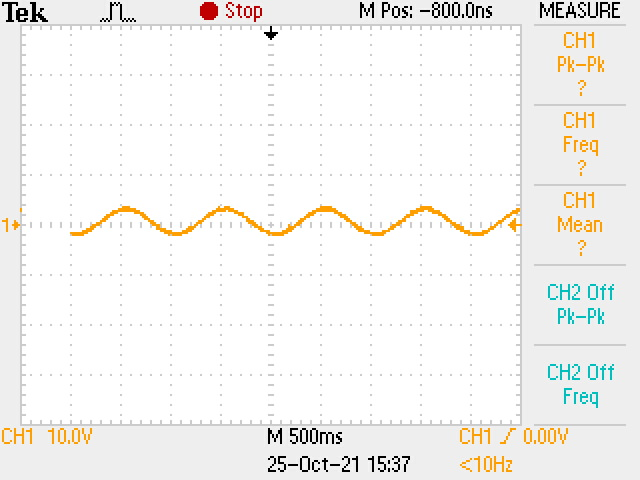
\includegraphics[width=\columnwidth]{img/testing/power_output/filter_output_1Hz.JPG}
      \subcaption{}
  \end{subfigure}
  \begin{subfigure}{0.3\textwidth}
      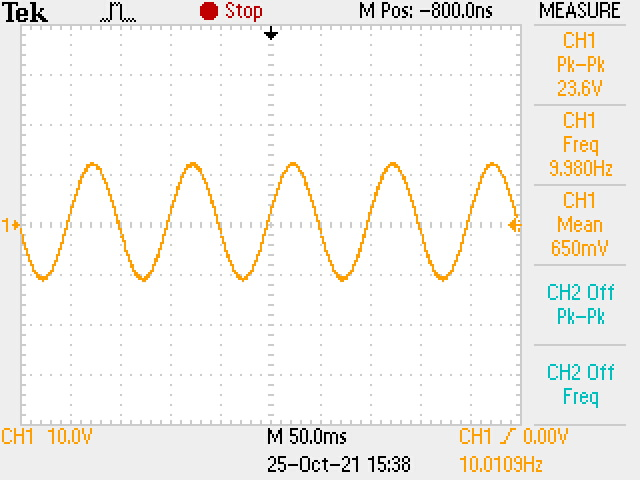
\includegraphics[width=\columnwidth]{img/testing/power_output/filter_output_10Hz.JPG}
      \subcaption{}
  \end{subfigure}
  \begin{subfigure}{0.3\textwidth}
      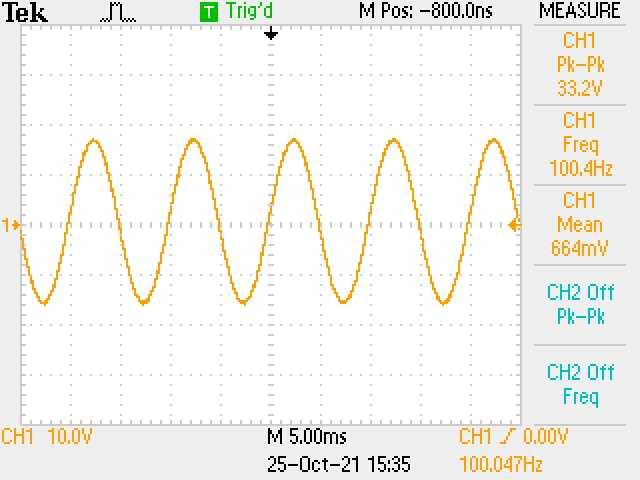
\includegraphics[width=\columnwidth]{img/testing/power_output/filter_output_100Hz.JPG}
      \subcaption{}
  \end{subfigure}
  \begin{subfigure}{0.3\textwidth}
      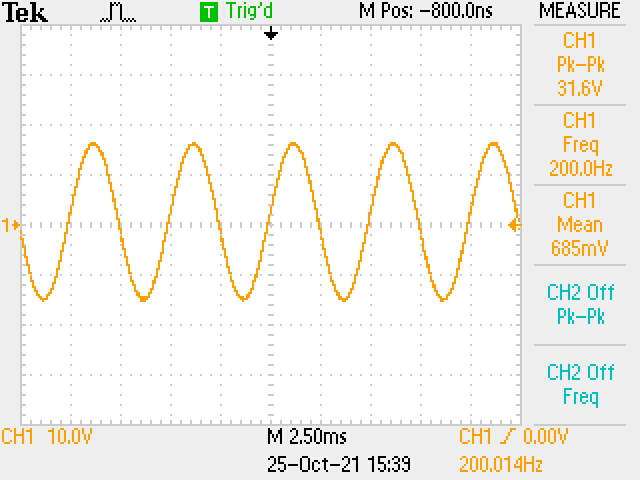
\includegraphics[width=\columnwidth]{img/testing/power_output/filter_output_200Hz.JPG}
      \subcaption{}
  \end{subfigure}
  \begin{subfigure}{0.3\textwidth}
      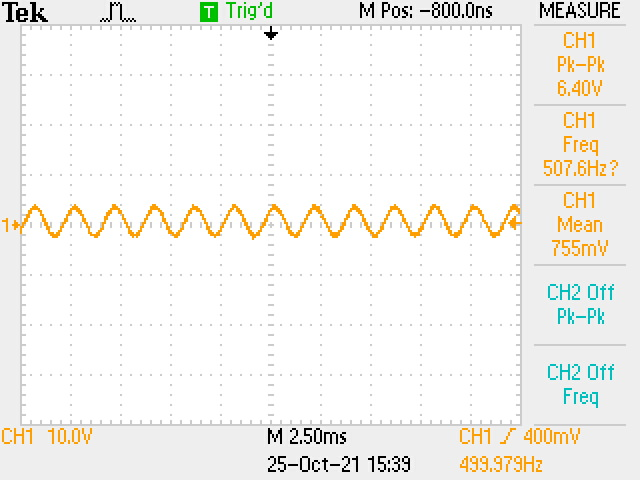
\includegraphics[width=\columnwidth]{img/testing/power_output/filter_output_500Hz.JPG}
      \subcaption{}
  \end{subfigure}
  \begin{subfigure}{0.3\textwidth}
      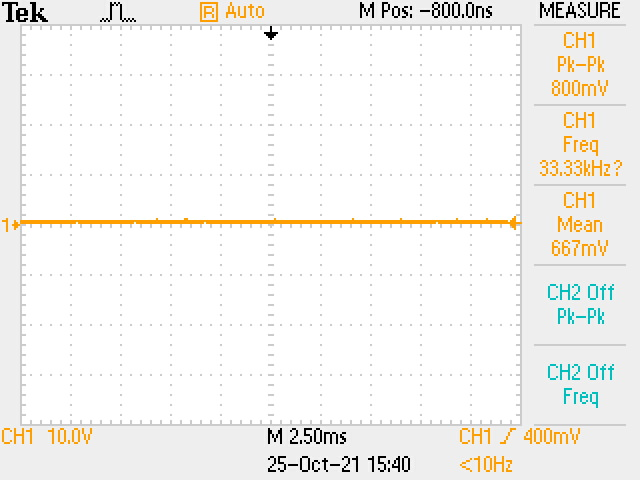
\includegraphics[width=\columnwidth]{img/testing/power_output/filter_output_2kHz.JPG}
      \subcaption{}
  \end{subfigure}
  \caption{Output from Reconstruction filter at various frequencies}
  \label{F:opt_filter_res}
\end{figure}

To show the reconstruction filter successfully removed the carrier frequency and retain the correct bandwidth attenuation to meet the specification in \cref{S:spec} the input signal was varied from 10Hz to 2kHz and the results are very successfully shown in \cref{F:opt_filter_res}.

\subsubsection*{Extra}
The only changes made in testing was the addition of an $100uF$ smoothing capacitor on the mid-rail voltage reference for the input signal processing to prevent oscillations. 

\newpage
\section{Results}

To finalise and summarise the overall performance of this Class D amplifier a series of frequency sweeps were undertaken and the measurements relevant to \cref{S:spec} were taken. 

\begin{figure}[h!]
  \centering
  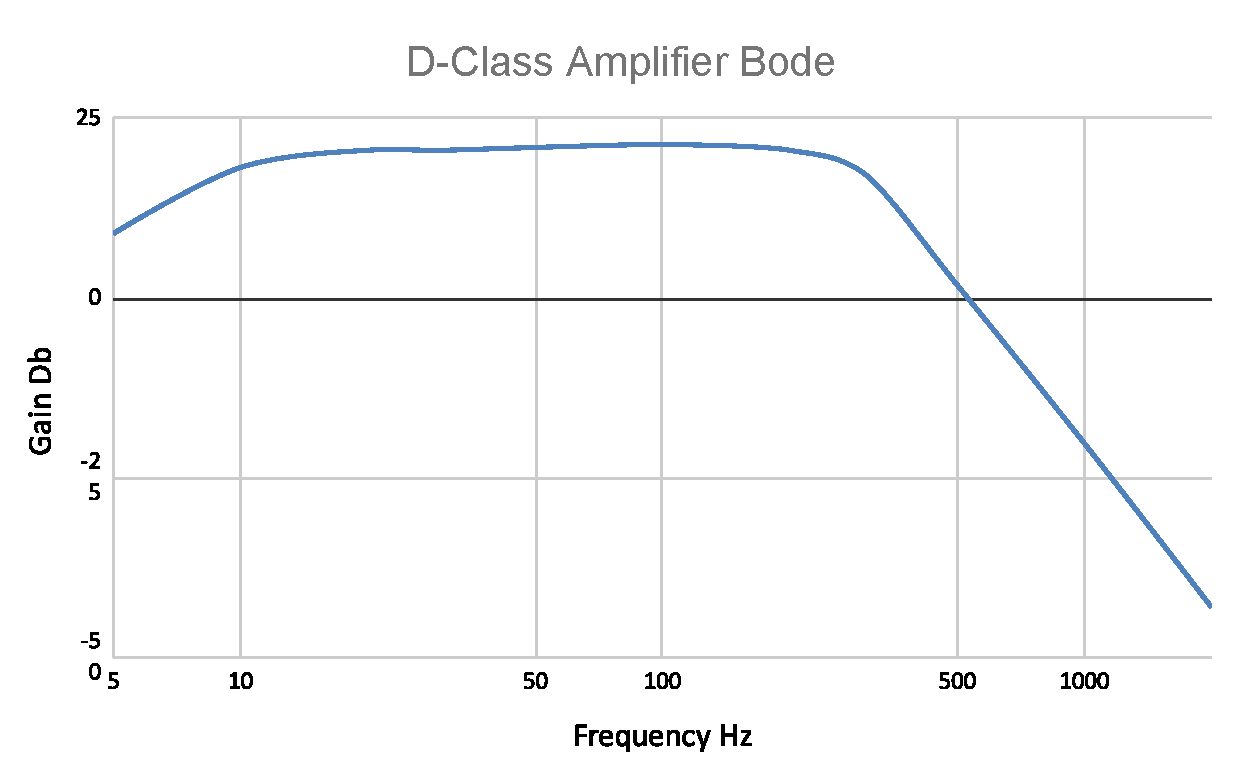
\includegraphics[width=0.75\textwidth]{img/testing/amplifier_bode.pdf}
  \caption{}
  \label{F:bode}
\end{figure}

By taking an FFT of the output signal (loaded) the Bode plot \cref{F:bode} shows a flat passband matching the 10Hz to 200Hz specification.

\begin{figure}[h!]
  \centering
  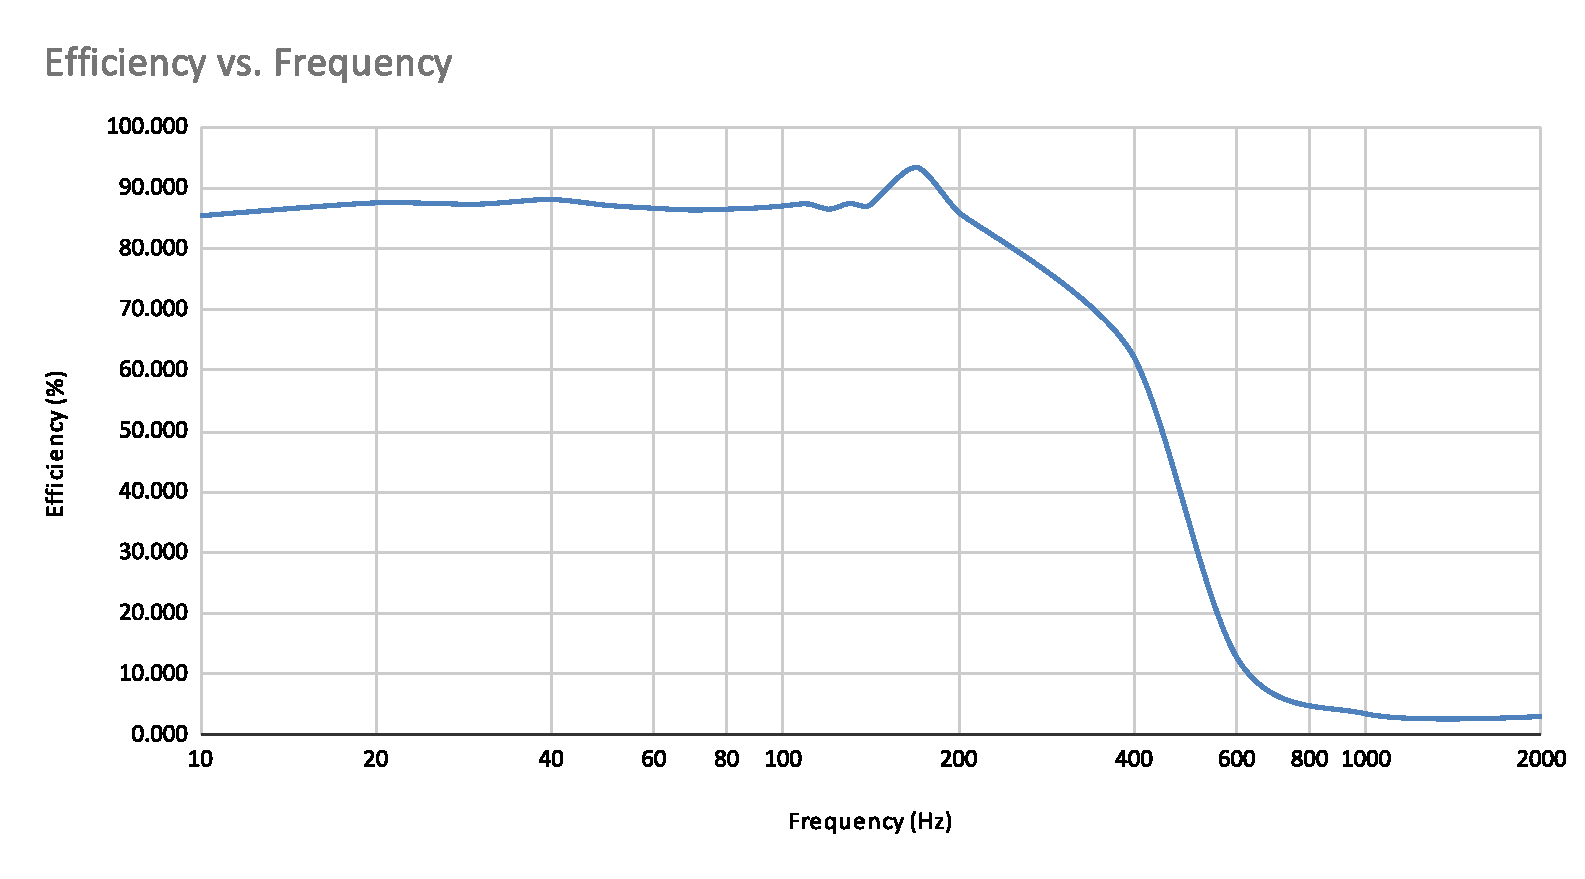
\includegraphics[width=0.75\textwidth]{img/testing/Efficiency_vs._Frequency.pdf}
  \caption{}
  \label{F:eff}
\end{figure}

\cref{F:eff} shows that by utilising the D class approach to power amplification, a very high efficiency could be achieved across the operating range. Sustaining 85\% to 95\%.  

\begin{table}[h!]
  \centering
  \begin{tabular}{l|l}
  \rowcolor[HTML]{E0E0E0} 
  \textbf{Frequency (Hz)} & \textbf{THD (\%)} \\ \hline
  30                 & 1.8               \\
  50                 & 2.2               \\
  100                & 3.2               \\
  200                & 3.3               \\
  300                & 3.5               \\
  500                & 3.2              
  \end{tabular}
  \caption{Output total harmonic distortion across frequency}
  \label{T:THD}
\end{table}

This \%THD was also measured across the measurable range (\cref{T:THD}) of the meter and shows what was approximately expected for a deadtime of 63ns. It could be possible to reduce this to sub \%1 by dropping down to 40ns but this was not explored.   

\newpage
\section{Conclusions}
 
In conclusion our segmented and thorough approach to design and careful layout consideration resulted in this project very successfully producing a D-Class amplifier to the given specifications in \cref{S:spec}. We were also able to maintain the \$50 per board cost and order and construct 3 working devices, outlined in this \href{https://niels-clayton.github.io/D-Class\_Amplifier/}{Interactive BOM}.

The feeling of which can be accurately summarised by \cref{F:thumbs}.
\begin{figure}[h!]
  \centering
  
\includegraphics[width=0.5\textwidth]{img/thumbs.png}  
  \caption{}
  \label{F:thumbs}
\end{figure}

\newpage
\section*{Appendix}
Implementation results of other team members stages.
\subsection*{Input Filter}
\begin{figure}[h!]
  \centering
  \begin{subfigure}{0.3\textwidth}
    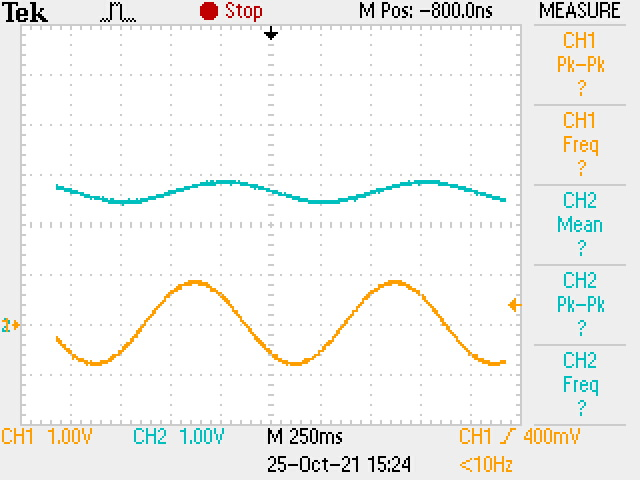
\includegraphics[width=\columnwidth]{img/testing/input_filter/input_1Hz.JPG}
    \subcaption{1Hz}
  \end{subfigure}
  \begin{subfigure}{0.3\textwidth}
    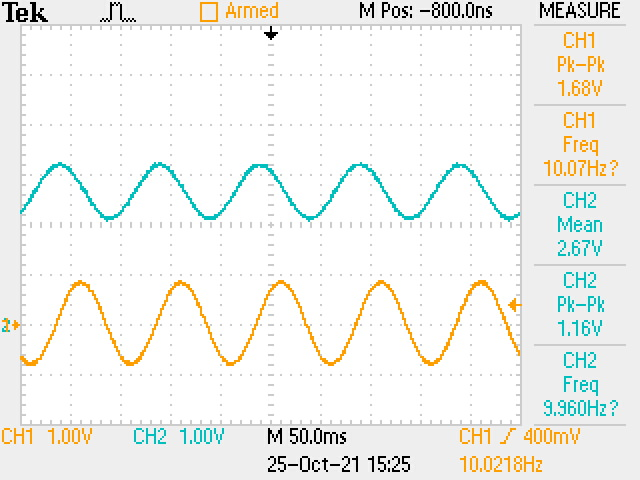
\includegraphics[width=\columnwidth]{img/testing/input_filter/input_10Hz.JPG}
    \subcaption{10Hz}
  \end{subfigure}
  \begin{subfigure}{0.3\textwidth}
    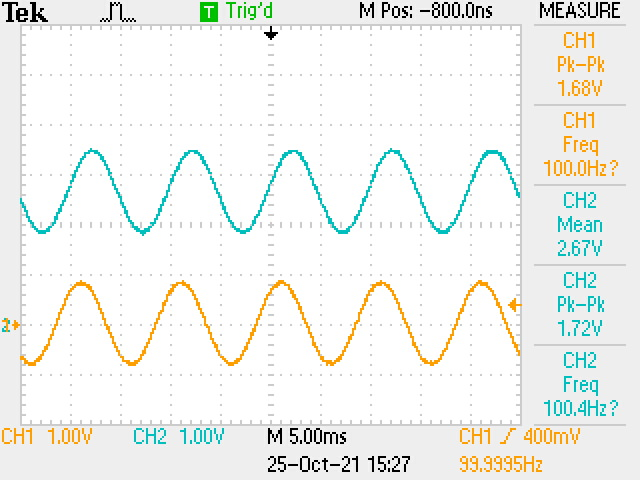
\includegraphics[width=\columnwidth]{img/testing/input_filter/input_100Hz.JPG}
    \subcaption{100Hz}
  \end{subfigure}
  \begin{subfigure}{0.3\textwidth}
    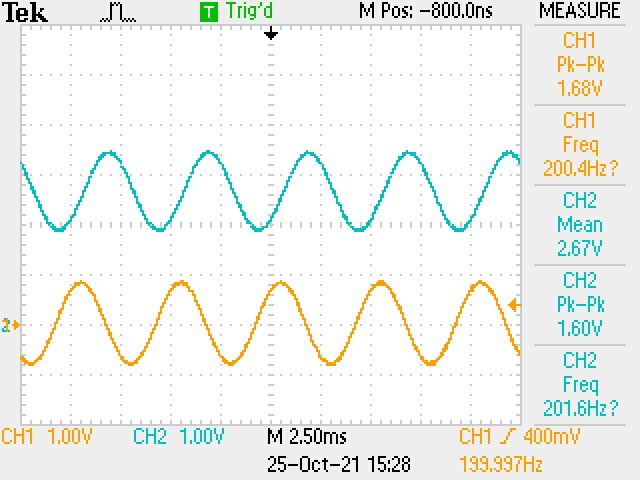
\includegraphics[width=\columnwidth]{img/testing/input_filter/input_200Hz.JPG}
    \subcaption{200Hz}
  \end{subfigure}
  \begin{subfigure}{0.3\textwidth}
    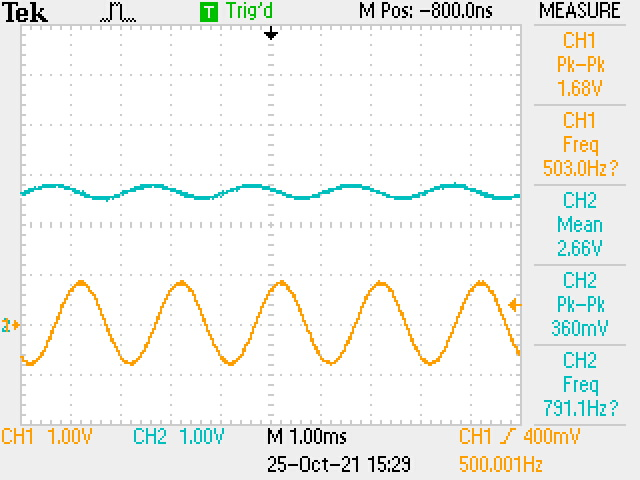
\includegraphics[width=\columnwidth]{img/testing/input_filter/input_500Hz.JPG}
    \subcaption{500Hz}
  \end{subfigure}
  \begin{subfigure}{0.3\textwidth}
    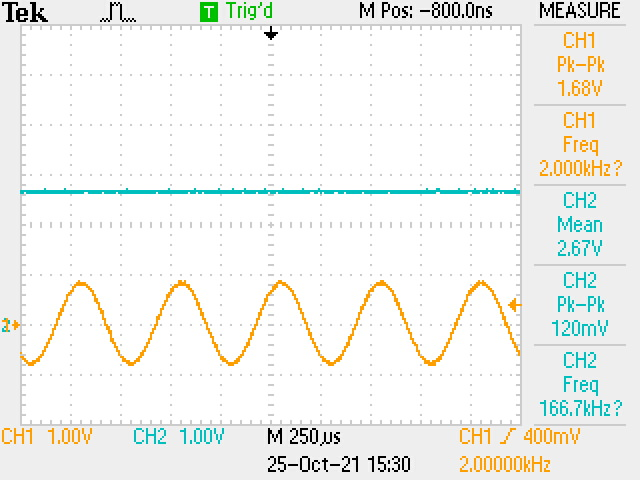
\includegraphics[width=\columnwidth]{img/testing/input_filter/input_2kHz.JPG}
    \subcaption{2kHz}
  \end{subfigure}
\end{figure}

\subsection*{Sampling/SPWM}
\begin{figure}[h!]
  \centering
  \begin{subfigure}{0.3\textwidth}
    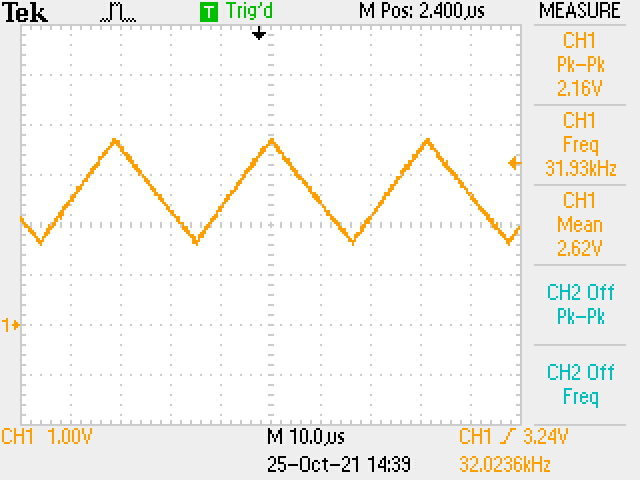
\includegraphics[width=\columnwidth]{img/testing/spwm/triangle_wave_32kHz.JPG}
    \subcaption{Triangle Qave}
  \end{subfigure}
  \begin{subfigure}{0.3\textwidth}
    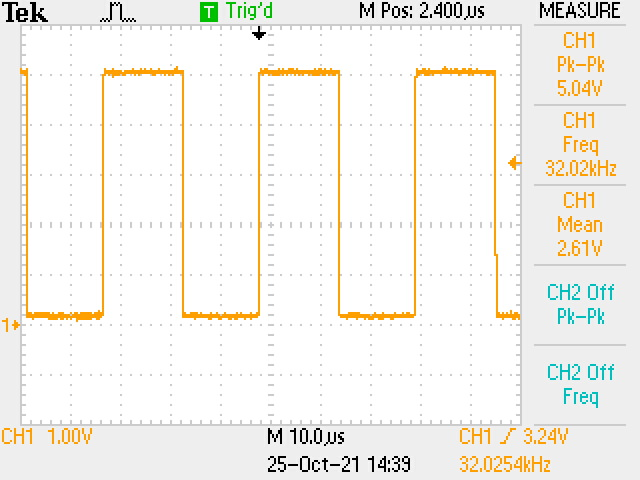
\includegraphics[width=\columnwidth]{img/testing/spwm/spwm_no_input.JPG}
    \subcaption{SPWM w/ 0V Input}
  \end{subfigure}\\
  \begin{subfigure}{0.3\textwidth}
    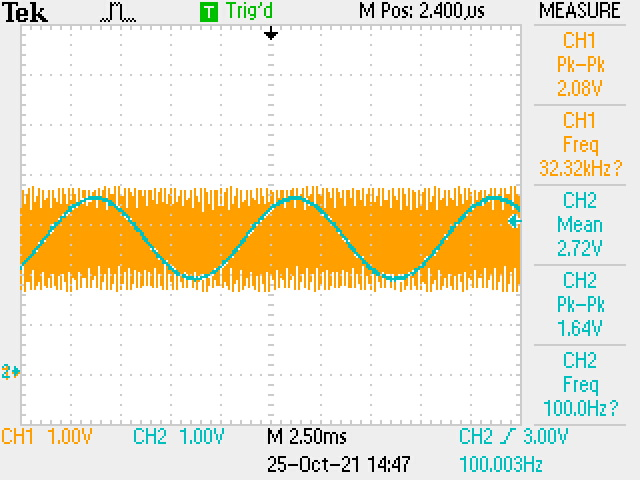
\includegraphics[width=\columnwidth]{img/testing/spwm/input_sampling_0.JPG}
    \subcaption{Input Signal Sampling Far}
  \end{subfigure}
  \begin{subfigure}{0.3\textwidth}
    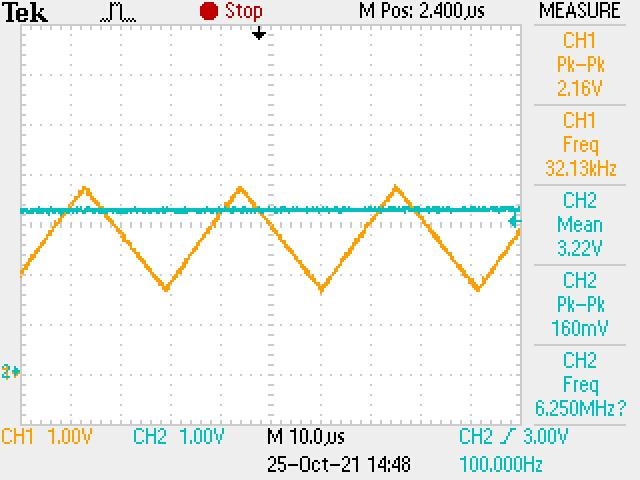
\includegraphics[width=\columnwidth]{img/testing/spwm/input_sampling_1.JPG}
    \subcaption{Input Signal Sampling Near}
  \end{subfigure}
\end{figure}

\end{document}